%!TEX root = ./main.tex

%-------------------------------------
%-------------------------------------
% The model
%-------------------------------------
%-------------------------------------
\section{The model}

%\subsection{The model}

\begin{frame}{Our model}

\alert{Goal}: given a set of $n$ data with $p$ variables, infer the block structure of their variables
without knowing the number of groups.

\pause

\alert{Additional constraints}: 
\begin{itemize}
    \item use a Stochastic Block Model    
    \item the partition must respect the original order of the variables
\end{itemize} 

\pause

\alert{The model}: 
\begin{align*}
    \bm{y}_1, \ldots, \bm{y}_n \mid \bm{K} & \iid \mathcal{N}_p(\mathbf{0}, \bm{K}^{-1} ) \\
    \bm{K} \mid G & \sim \GWish(b, D)\\
    P((i,j)&\in E\mid \bm{z},Q) = Q_{z_{i} z_{j}},\,\text{independent}\\
        Q_{rs} \mid \bm{z} &\ind \Beta(a,b), 1\leq r\leq s\leq H\\
    \rho_p & \sim \mathcal{L}\left(\rho_p\right)
\end{align*}

% TODO inserire la prior?

\end{frame}


%-------------------------------------
%-------------------------------------
% The sampling strategy
%-------------------------------------
%-------------------------------------
\section{The sampling strategy}

\subsection{Overview of the sampling strategy}
\begin{frame}{Block Gibbs Sampler}
    Full conditional distributions for our model:
    \begin{itemize}
        \item Precision Matrix: $P(\bm{K} \mid \bm{Y},G,\bm{z}) \propto P(\bm{Y} \mid \bm{K})P(\bm{K} \mid {G})$ 

        \item Graph: $P(G \mid \bm{Y},\bm{K},\bm{z}) \propto P(\bm{Y} \mid \bm{K})P(\bm{K} \mid {G})P(G \mid \bm{z})$ 

        \item Random Partition: $P(\bm{z} \mid \bm{Y},\bm{K},G) \propto P(\bm{Y} \mid \bm{K})P(\bm{K} \mid {G})P(G \mid \bm{z})P(\bm{z}) \propto P(G \mid \bm{z})P(\bm{z}) $
    \end{itemize}

    \pause 

    We implement a Block Gibbs-Sampler strategy:
    \begin{enumerate}
        \item \alert{Sampling Graph and Precision Matrix}\\
        $G$ and $\bm{K}$ - given $\bm{z}$ - are sampled using a modified version of a Birth-and-Death chain, changing one link at a time
        \item \alert{Sampling the Random Partition}\\
        We can sample $\bm{z}$ through an adaptive MCMC\vphantom{changepoint} sampler, working conditionally on $G$ after the graph update
    \end{enumerate}
\end{frame}




%-------------------------------------
% BDgraph
%-------------------------------------
\subsection{Updating the graph}
\begin{frame}{Birth and death algorithm for updating the graph}

    \texttt{BDGraph} is an algorithm that follows a Birth-and-Death approach to decide whether to \alert{add} a new edge to the graph or \alert{delete} an already existing one.

    How did we change it?

    \pause
    
    % https://people.inf.ethz.ch/markusp/teaching/guides/guide-tables.pdf
    \begin{table}[tb]
        \centering
        \begin{tabular}{lcc}
        \toprule
        & Conditional & B/D rates \\ % TODO Full conditional non è il termine giusto, join conditional?
        \hline
        \textbf{Before} & $P(G,\bm{K} \mid \bm{Y}) \propto \mathcal{L}(\bm{Y} \mid \bm{K})\mathcal{L} (\bm{K} \mid {G})P(G)$ & $\cfrac{P(G')}{P(G)}$ \\
        \textbf{After}  & $P(G,\bm{K} \mid \bm{Y}, \textcolor{sleekRed}{\bm{z}}) \propto \mathcal{L}(\bm{Y} \mid \bm{K})\mathcal{L}(\bm{K} \mid {G})P(G \mid \textcolor{sleekRed}{\bm{z}})$ & $\cfrac{P(G' \mid \textcolor{sleekRed}{\bm{z}})}{P(G \mid \textcolor{sleekRed}{\bm{z}})}$ \\
        \bottomrule
        \end{tabular}
    \end{table}
    where $G' = G^{\pm e}$ and $e$ is an edge.
    \pause
    %We computed the birth and death rates as:
    \[
        \text{Birth rate} = \frac{P(G^{+ e}\mid \bm{z})}{P(G\mid \bm{z})} = \frac{S_{uv} + a}{T_{uv} - S_{uv} + b}
        \quad
        \text{Death rate} =\frac{P(G^{- e}\mid \bm{z})}{P(G\mid \bm{z})} = \frac{T_{uv} - S_{uv} + b}{S_{uv} + a}
    \]
    % TODO l'utente non sa cosa siano T,S,a,b forse si potrebbe balzare
    
\end{frame}


%-------------------------------------
% Updating the current partition
%-------------------------------------
\subsection{Updating the partition}


\begin{frame}{General steps for updating the partition}
    
    We perform an (adaptive) \alert{split and merge} as in \cite{bensonAdaptiveMCMCMultiple2018}.
    \begin{enumerate}
        \item With probability $\alpha_{\text{split}}$, usually $0.5$, choose an \alert{split move}, otherwise a \alert{merge move}. Unless we are forced by extreme cases.
        \begin{enumerate}
            \item Propose a new partition by splitting one group into two or merging two adjacent ones.
            \item Accept or reject using Metropolis Hastings. The target is:
            $f(\rho \mid G) \approx f_G(G \mid \rho) f_{\rho}(\rho)$
            \[
                \alpha_{\text{accept}} = \min
                \bigg\{1,
                \overbrace{
                \underbrace{\frac{f_G\left(G \mid \rho'\right)}{f_G(G \mid \rho)}}_{\substack{\text{likelihood}\\\text{ratio}}}
                \underbrace{\frac{f_\rho\left(\rho'\right)}{f_\rho(\rho)}}_{\substack{\text{prior}\\\text{ratio}}}
                }^{\text{target ratio}}
                \underbrace{\frac{Q(\rho',\rho)}{Q(\rho,\rho')}}_{\substack{\text{proposal}\\\text{ratio}}}
                \bigg\}
            \]
        \end{enumerate}
        \item To improve the mixing of the chain we also perform a \alert{shuffle move}.
        \begin{enumerate}
            \item Propose a new partition by moving some nodes from a group to an adjacent one.
            \item Accept or reject using Metropolis Hastings.
        \end{enumerate}

    \end{enumerate}

\end{frame}

\begin{frame}{Visual explanation of the possible partition updates}
    \fg{1}{update_partition.pdf}
\end{frame}







\begin{frame}{Proposal ratio}

We introduce $\bm{a}^{(t)}$ and $\bm{d}^{(t)}$, two $p$-dimensional vectors of \alert{weights} to choose the node where to perform the split or the merge. They are unnormalized discrete densities.

\pause

Suppose a merge move.

\pause

At each iteration, \alert{draw} node $i$ proportionally to $d_{i}^{(t)}$.

\pause

Denoting by $a^{\star} = \sum_{j\in \{\text{admissible split nodes}\}}{a_{j}^{(t)}}$ and $d^{\star} = \sum_{j\in \{\text{admissible merge nodes}\}}{d_{j}^{(t)}}$

\pause

\[
    \frac{Q(\rho',\rho)}{Q(\rho,\rho')}
    =
    \frac{P(\text{choose merge})}{P(\text{choose split})}
    \cdot 
    \frac{P(\text{merge at node $i$})}{P(\text{split at node $i$})}
    =
    \frac{1-\alpha_{\text{split}}}{\alpha_{\text{split}}}
    \cdot
    \frac{\frac{a_{i}^{(t)}}{a^{\star}+a_{i}^{(t)}}}{\frac{d_{i}^{(t)}}{d^{\star}}}
\]
The extreme cases ``every node belonging to the same group'' and ``every node has its own group'' are dealt with separately.

\end{frame}




\begin{frame}{Adaptive step}
    The two weights vectors $\bm{a}^{(t)}$ and $\bm{d}^{(t)}$ are updated at each iteration $t$ as in \cite{bensonAdaptiveMCMCMultiple2018} using the following 
    \textbf{adaptation scheme}.

    \begin{itemize}
        \item If a \alert{split} move at node $i$ has been accepted then update:
		\[
		\log (a_i^{(t+1)})=\log (a_i^{(t)})+\frac{h}{t / n}(\alpha_{\text{split}}-\alpha_{\text{target}}) .
		\]
        \item If a \alert{merge} move at node $i$ has been accepted then update:
		\[
		\log (d_i^{(t+1)})=\log (d_i^{(t)})+\frac{h}{t / n}(\alpha_{\text{del}}-\alpha_{\text{target}}) .
		\]
        \end{itemize}
Where $h>0$ is the initial adaptation and $t/n$ are the iterations $(t)$ per number of datapoints $(n)$.
%TODO il numero di osservazioni, giusto?

\end{frame}



%-------------------------------------
%-------------------------------------
% Next steps
%-------------------------------------
%-------------------------------------
\section{Next steps}
\begin{frame}{Next steps}

    \begin{itemize}
        \item Praying that the code works
    \end{itemize}



% TODO chiedere a colombi quanta roba extra mettere e se inserire il discorso sul grafo finale e partizione finale (a proposito, qual è la partizione finale?)

\end{frame}



%----------------------------------------
% References
%-------------------------------------

\begin{frame}{Main references}
    % GGM
    \nocite{colombiLearningBlockStructured2022a}
    \nocite{mohammadiBayesianStructureLearning2015a}
    % SBM
    \nocite{legramantiExtendedStochasticBlock2022}
    % Changepoint
    \nocite{bensonAdaptiveMCMCMultiple2018}
    \nocite{martinezNonparametricChangePoint2014}
    
    
    %biblatex
    \printbibliography
    \renewcommand*{\bibfont}{\small}
    %bibtex
    %\bibliographystyle{plain} % We choose the "plain" reference style
    %\bibliography{bibliography} % Entries are in the refs.bib file
\end{frame}



\begin{frame}[plain]
    % Add background to content page
    \AddToShipoutPictureFG*{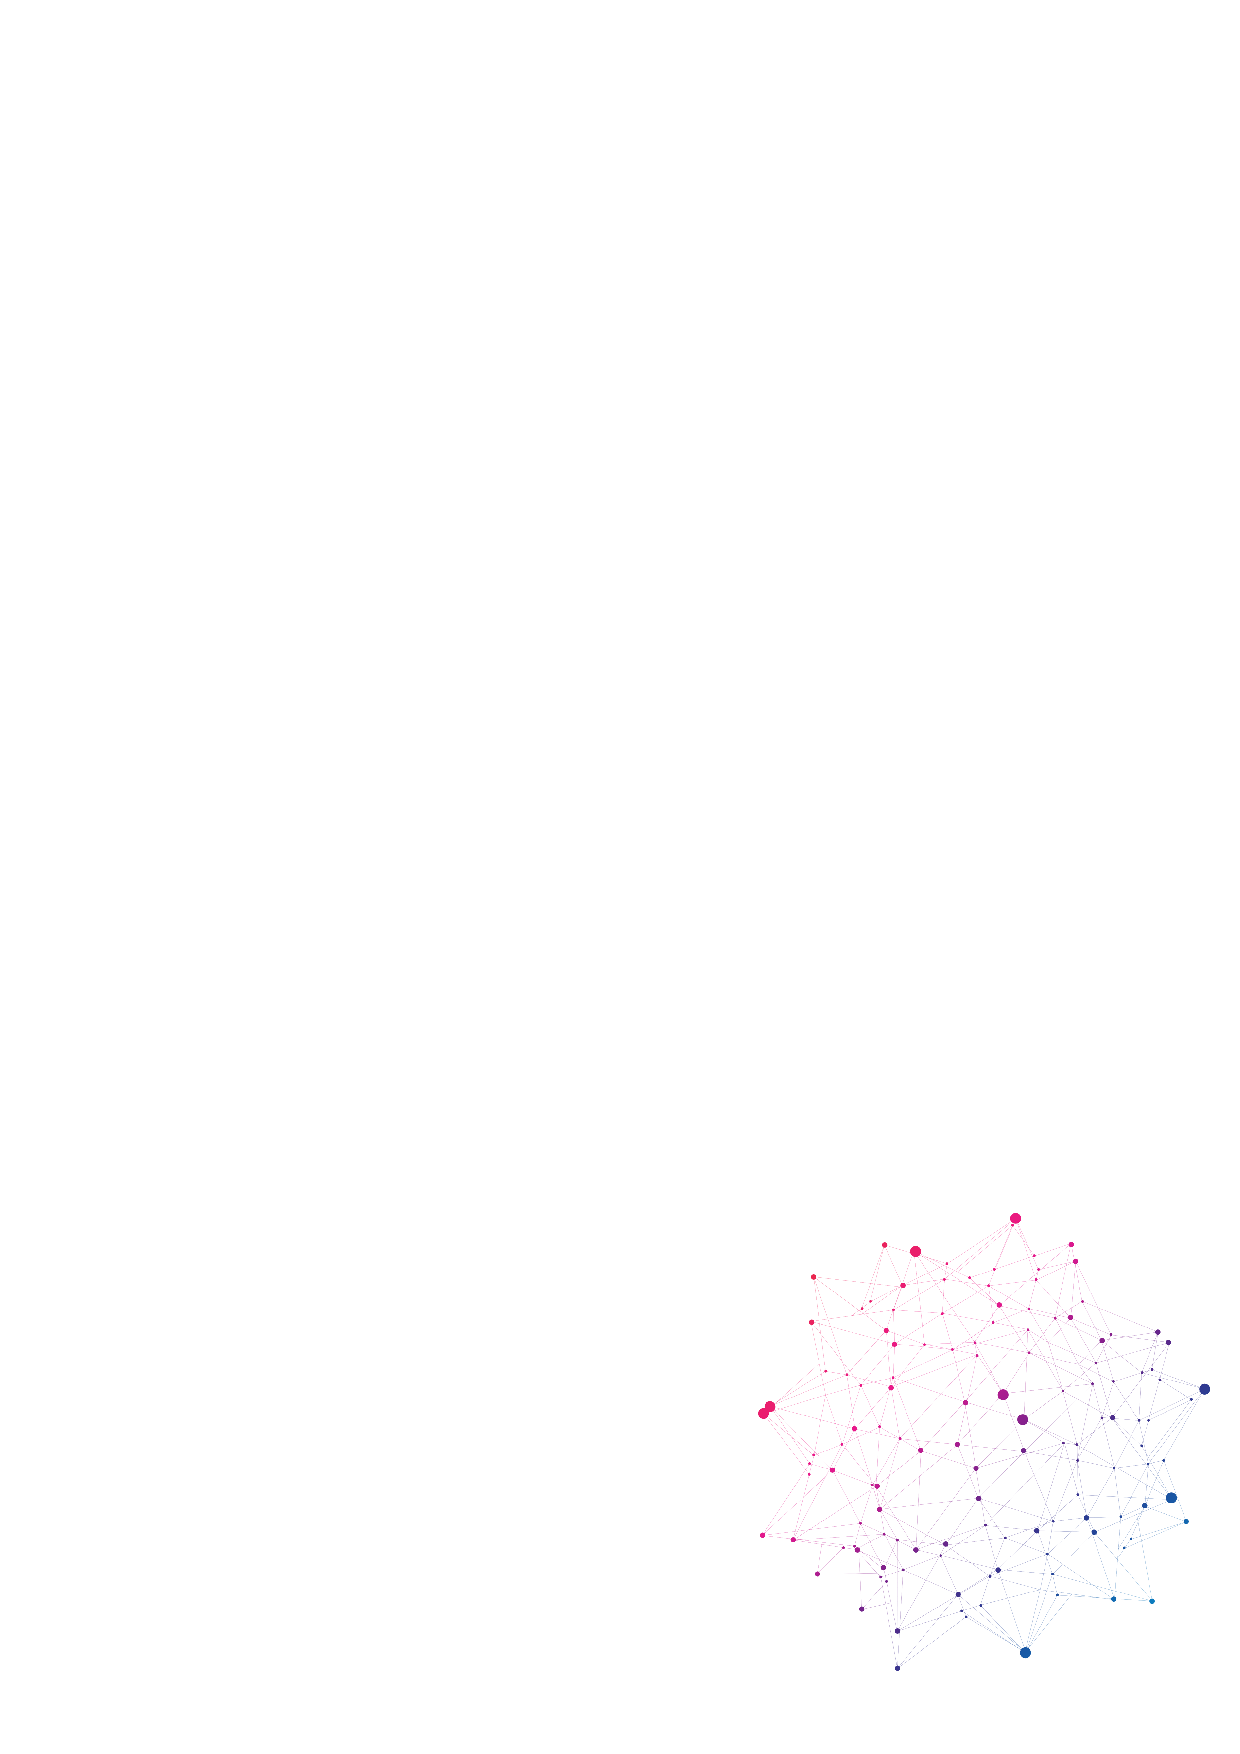
\includegraphics[width=\paperwidth]{Images/background.pdf}}
    \vspace*{1.2cm}
    \hspace*{1cm}{\Large Thank you!}\\
    \vspace*{0.6cm}
    \hspace*{1cm}{\Huge \alert{Any questions?}}
\end{frame}





%tenere?
\section*{Extra}

\begin{frame}{Extra content}


\end{frame}


